%% conclusion.tex
%%

%% ==================
\chapter{Conclusion}
\label{ch:Conclusion}
%% ==================

In this section, the conclusions from the evaluation section are drawn and potential limitations of the result are discussed. Furthermore, lessons learned from the experiment are described and potential fields of further research are examined.


\paragraph{\acf{AMT} and the quality of data}
As indicated by the findings of the \acl{NP}, the data generated on \ac{AMT} includes a lot of noise. Many participants failed to get a result higher than 80\%, a level which can be considered as fairly easy to achieve. Even increasing the leverage of the bonus and the total possible payout did not show to have an influence on the participants. So we must conclude, that offering the experiment as a \ac{HIT} on \ac{AMT} will return a lot of data that is not usable for the analysis of statistical implications. The advantages of a computer-lab experiment clearly lay in the quality of the data.

\paragraph{Information Granularity and its influence on the \textit{FirstResult} and \textit{DecisionTime}}
When focusing the statistical analysis on the participants who took an effort to succeed in the game, the statistical results get clearer. The hypothesis, that the highest performance will be achieved on a medium level of information granularity is supported for the first result that the participants offer. These findings are in particular interesting because we argue that users of smart meters divide their time between many things, and are interested in achieving a satisfying result in a minimum time.\\
The findings for the \textit{DecisionTime} indicate that users facing a medium level of granularity take the most time to make a decision. These results are supported by \citep{Jacoby1974} who argues that individuals facing a higher information overload are selective in their information selection. When confronted with too much information, they only concentrate on one part and do not include all the available information to make their choices. A participant on a medium level of information granularity is just at the border of information overload - the individual can still cope with the amount of information, and since the information provides more detail than on a lower level of the information granularity, the choice is supported by a better understanding of the underlying parameter (Benefit).\\
In addition, when excluding the lower levels of information granularity, the results of the statistical model indicate that the best performance can be achieved on a medium-to-high level of information granularity. These findings are not described in our original hypothesis, but have implications for the further development of the experiment. \textbf{TO DOO!!!}

\paragraph{Learning Effect}

Participants did improve their performance with a growing number of played rounds, even tough the learning effect diminishes over the number of rounds. So we can conclude that individuals find strategies to cope with information overload when they get more experienced in this situation. A potential question to ask for future is how these findings are reflected in a setup that includes more rounds.

\paragraph{Individual Influence on the performance}
Individual characteristics has proven to be influential on the participants. Even tough participants might show a similar sensitivity to the level of information granularity, their performances is affected by many individual factors that are not part of our research. Taking into account these effects when setting up a statistical model helps us to exclude influences such as limited attention while playing the game or a individual talent for succeeding in these types of experiments. So limitations of the \acl{AMT} must not only be considered during the design of the experiment, but the statistical model has to be adjusted to the characteristics of the \ac{AMT}.



One reason for the lack of a detectable learning effect might be the trial round prior to the game. This opportunity enabled the participants to spend as much time as desired on exploring the experiment and on trying different strategies. As indicated by the timelog analysis in Section \ref{ch:Experiment:sec:DataacquisitionDescriptives}, the participants spent the majority of their time on the explanation part and used the chance to get familiar with the experiment. The trial round was necessary to ensure that participants were fully aware of the task and the design of the experiment. Yet, the learning curve already started here, participants could improve their performance without any time pressure and were used to the implemented information overload. The findings for the final performance from Round 1 and 2 might be an indication that the learning effect continued for the first 2 rounds. Having said that, one would expect the final performance for Round 3 to be at least the level of the performance in Round 2, yet usergroup 3 and 4 reduce their performance in Round 3.\\
The lack of a learning effect is interesting since prior research with a similar experiment \citep{Schmidt2012} gave an indication that a learning effect is significant. In contrast to our setup, Schmidt's experiment included 13 runs, so 

excluding those participants who were not able to perform better than 80\%


As indicated by the findings of the \acl{NP}, the data generated on \ac{AMT} includes a lot of noise. Many participants failed to get a result higher than 80\%, a level which can be considered as fairly easy to achieve. Even increasing the leverage of the bonus and the total possible payout did not show to have an influence on the participants. So we must conclude, that offering the experiment as a \ac{HIT} on \ac{AMT} will return a lot of data that is not usable for the analysis of statistical implications. The advantages of a computer-lab experiment clearly lay in the quality of the data.




\section{Information Granularity}

The influence of the information granularity has not shown the expected magnitude since all the related hypotheses are rejected. Nevertheless, a comparison between a low information granularity and a high information granularity - usergroup 1 and 4 - returns significant results, indicating, that a low information granularity leads to better choice accuracy. 

In order to back up these findings, further research might add more colours to the framework to prove the negative correlation between number of colours and performance. A small change for the number of colours between treatments did not emerge to be the right approach to get distinctive results for each treatment, so we would suggest to increase the number of colours with a larger step size, e.g. introducing 27 or more colours. This approach might be more successful in finding a significant relationship between information granularity and choice accuracy.\\
Yet, the reason for the lack of significant results for a medium information granularity must be further discussed. When the number of colours is increased, two opposing trends in the complexity of the game can be identified. As the number of colours increases, the color frame gets more complex and the dimension of the attribute level \textit{benefit} increases. This development reinforces the information load, as indicated by \cite{Jacoby1974} and \cite{Malhotra1982}. In contrast to that, with a growing number of colours, the benefit range covered by one colour decreases, so the choices get more specific and accurate. Whereas participant 1 who faces a low number of colours can choose between colours that represent a wide range of benefit, participant 2 who is challenged with a high number of colours can choose among colours that represent a more specific benefit value. Consequently, the participant 2 is less dependent on the chance that he or she clicks a box with a high benefit within the benefit range, but can make a more conscious choice.\\
These two opposing trends might be one reason why there is no clear development detectable for increasing number of colours. Reducing the complexity of the game to a controllable, one-dimensional approach would be a potential for future research. In the forefront of the experiment, several interfaces were open for discussion. The implemented approach was chosen because it guaranteed the comparability among usergroups, since the underlying knapsack problems are the same. If future research finds a way to combine comparability and one-dimensional complexity, the findings might get clearer for the influence from information granularity. One approach would be to assign one specific value per colour. This will result in different benefit ranges for each treatment and challenge the comparability of the problems. Yet, by using the delta-benchmark that was applied for the comparability between rounds, researchers can control the difficulty of the underlying problems and can consequently control comparability.

\section{Learning Effect}



\section{Limitations of the experiment}
As stated in Section \ref{ch:Evaluation:sec:DescriptiveStatistics:subsec:Distributionofusergroups}, the distribution of participants among usergroup was not uniformly. Since we saw a higher dropout-rate for usergroups with a higher number of colour, the representation of the population mean in each usergroup might be diluted. As participants drop out of usergroups 2, 3 and 4, the data is skewed towards participant in usergroup who face a lower information load. Our findings would be therefore suspect, if the performance of usergroup 1 was worse than the performance of all usergroups since the better performance of usergroup 2, 3 and 4 might be related to the dropout of participants who were unable to cope with the information overload.

Oversimplification of information overload experiments 433 \cite{Jacoby1984}

Control group with 3, 7, 11, 15

No Random treatment assignment!! ==> No representation of population mean
\dots



\begin{table}[p]%
\centering
\parbox{0.4\textwidth}{
\begin{footnotesize}
\begin{tabular}{l D{.}{.}{3.5} @{}}
\toprule
                 & \multicolumn{1}{c}{Parameters} \\
\midrule
(Intercept)      & -4.08^{\cdot} \\
                 & (1.90)        \\
NumberOfColours  & 1.84^{**}     \\
                 & (0.59)        \\
NumberOfColours2 & -0.10^{*}     \\
                 & (0.03)        \\
\midrule
R$^2$            & 0.49          \\
Adj. R$^2$       & 0.41          \\
Num. obs.        & 15            \\
\bottomrule
\vspace{-3mm}\\
\multicolumn{2}{l}{\textsuperscript{***}$p<0.001$, 
  \textsuperscript{**}$p<0.01$, 
  \textsuperscript{*}$p<0.05$, 
  \textsuperscript{$\cdot$}$p<0.1$}
\end{tabular}
\end{footnotesize}
\caption{Parameter estimations}
\label{tab:table}
}
\qquad
\begin{minipage}[c]{0.4\textwidth}%
\centering
    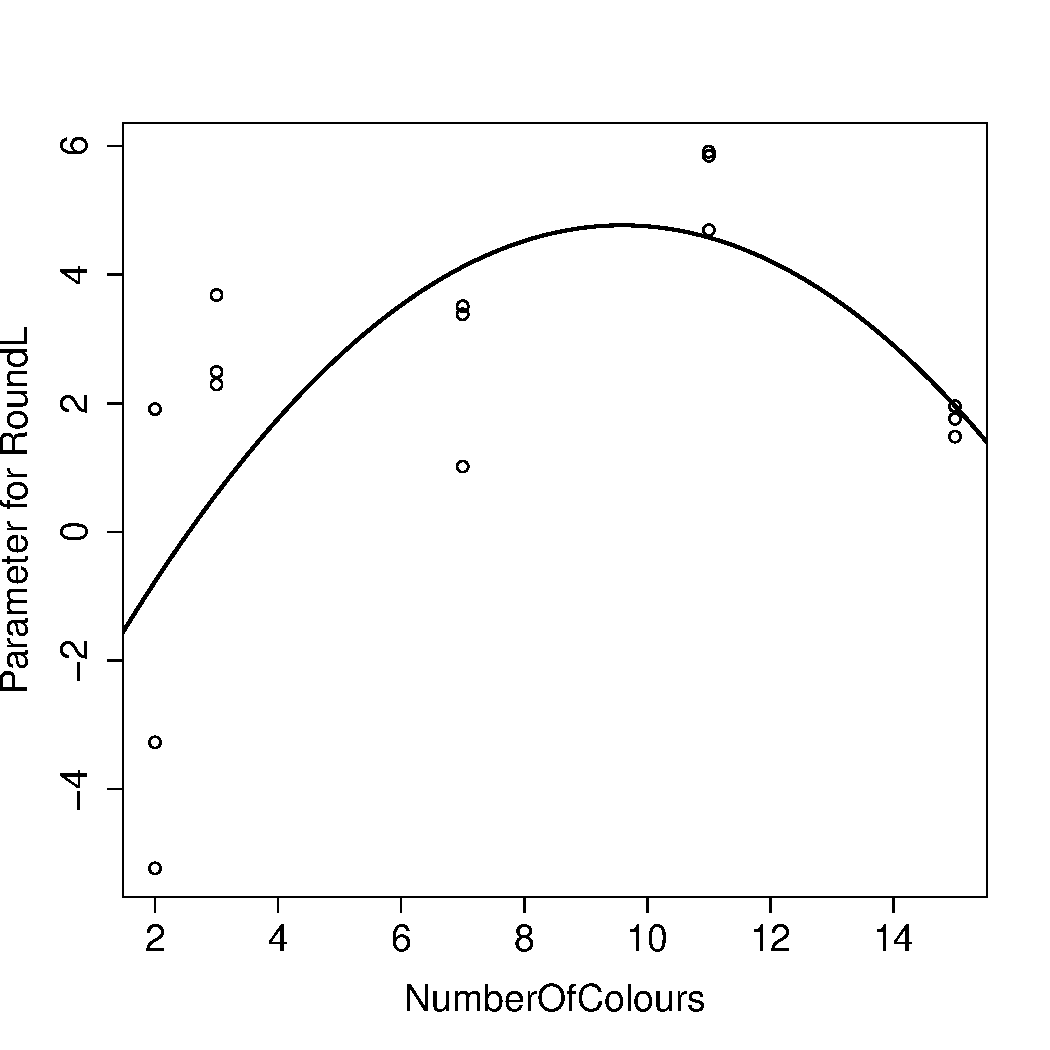
\includegraphics[width=1\textwidth]{PlotColoursLearningEffect.pdf}
\caption{Plot Parameters over NumberOfColours}
\label{fig:figure}
\end{minipage}
\end{table}